\subsection{Alta, baja y modificación de datos (ABMs)}
Para poder acceder al menú de configuración de datos el usuario actual debe tener el rol de administrador. En caso contrario dicho menú permanecerá oculto.

\begin{figure}[h]
\centerline{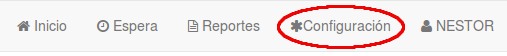
\includegraphics[width=0.7\textwidth]{menu_configuracion_visible.png}}
\caption{Menú de configuración visible}
\end{figure}

\begin{figure}[h]
\centerline{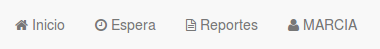
\includegraphics[width=0.7\textwidth]{menu_configuracion_oculto.png}}
\caption{Menú de configuración oculto}
\end{figure}

\subsubsection{ABM de síntomas}
Para acceder a la pantalla de administración de síntomas dirigirse hacia ''Configuración'' y luego a ''Síntomas''.

\begin{figure}[h]
\centerline{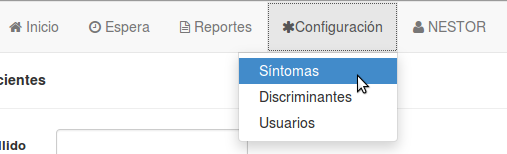
\includegraphics[width=0.7\textwidth]{menu_sintomas.png}}
\caption{Menú de síntomas}
\end{figure}

Cuando hacemos click en ''Síntomas'' se nos muestra el listado de todos los síntomas cargados en el sistema.

\begin{figure}[h]
\centerline{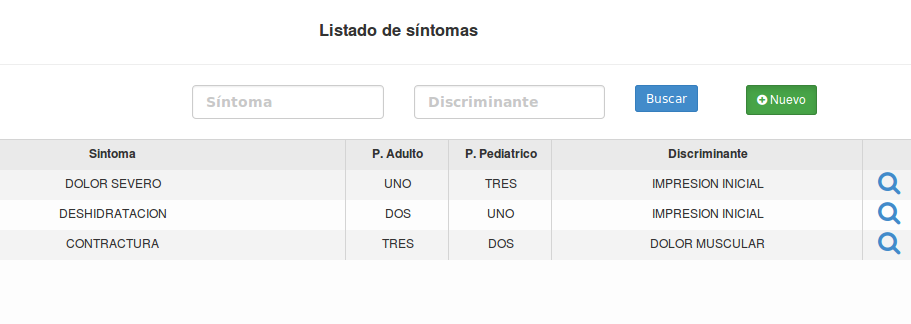
\includegraphics[width=1\textwidth]{sintomas_listado.png}}
\caption{Listado de síntomas}
\end{figure}

\subsubsection{Filtrado del listado}
Para facilitar la búsqueda de un síntoma podemos filtrar el listado llenando los campos de ''Síntoma'' y/o ''Discriminante''\footnote{El filtrado de los listados de síntomas, discriminantes y usuarios funciona de la misma manera. Por lo tanto en este manual sólo se explicará el filtrado del listado de síntomas}. No hace falta ingresar la palabra entera. Es suficiente con ingresar las primeras letras. No se distinguen mayúsculas y minúsculas. Luego de ingresar el valor deseado hay que hacer click en el botón ''Buscar''

\begin{figure}[h]
\centerline{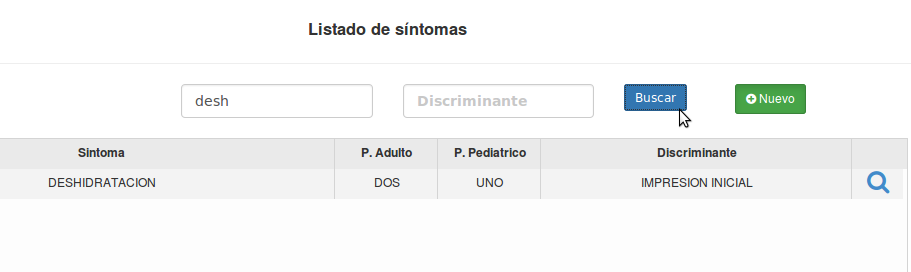
\includegraphics[width=1\textwidth]{sintomas_listado_filtro.png}}
\caption{Listado de síntomas filtrado}
\end{figure}

